\begin{figure}[H]
\centering
	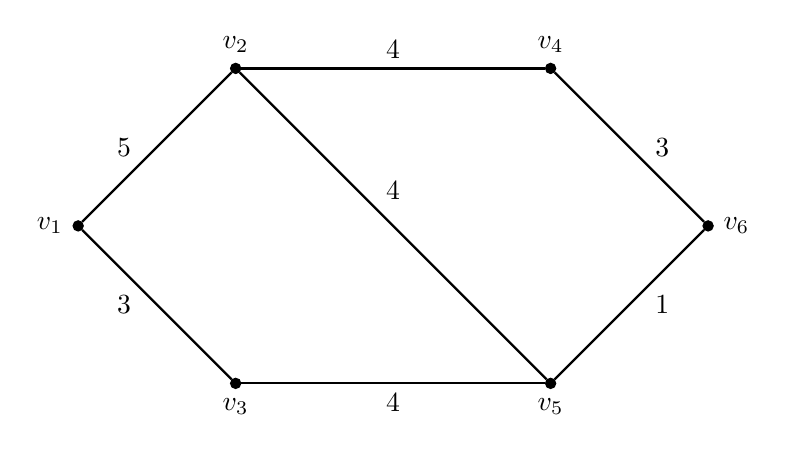
\begin{tikzpicture}

      \tikzset{enclosed/.style={draw, circle, inner sep=0pt, minimum size=.13cm, fill=black}}
%% Vertices
      	\node[enclosed, label={left: $v_1$}] (v1) at (0,2) {};
      	\node[enclosed, label={above: $v_2$}] (v2) at (2,4) {};
    	\node[enclosed, label={below: $v_3$}] (v3) at (2,0) {};
  	    \node[enclosed, label={above: $v_4$}] (v4) at (6,4) {};
     	\node[enclosed, label={below: $v_5$}] (v5) at (6,0) {};
     	\node[enclosed, label={right: $v_6$}] (v6) at (8,2) {};
%Edges
		\path [-, > = latex, thick] (v1) edge node[midway, left=2mm] {$ 5 $} (v2);
		\path [-, > = latex, thick] (v1) edge node[midway, left=2mm] {$ 3 $} (v3);
		\path [-, > = latex, thick] (v2) edge node[midway, above] {$ 4 $} (v4);
		\path [-, > = latex, thick] (v2) edge node[midway, above=2mm] {$ 4 $} (v5);
		\path [-, > = latex, thick] (v3) edge node[midway, below] {$ 4 $} (v5);
		\path [-, > = latex, thick] (v4) edge node[midway, right=2mm] {$ 3 $} (v6);
		\path [-, > = latex, thick] (v5) edge node[midway, right=2mm] {$ 1 $} (v6);

	\end{tikzpicture}
	\caption{Simpel, vægtet graf.}
	\label{fig.dijkstraexmp}
\end{figure}